% Perpendicular bisectors of a triangle
% Author: Sam Britt
%\documentclass[tikz,border=10pt]{standalone}
%%%<

%%%>
\begin{comment}
:Title: Perpendicular bisectors of a triangle
:Tags: Coordinate calculations;Foreach;Mathematical engine;Geometry;Mathematics
:Author: Sam Britt
:Slug: bisector

A perpendicular bisector of a line segment is a line which is perpendicular
to this line and passes through its midpoint. This drawing shows
perpendicular bisectors of a triangle. They meet in the center of the
circumcircle of the triangle.

This example was written by Sam Britt answering a question on TeX.SE.
\end{comment}
\usetikzlibrary{calc}
%\begin{document}
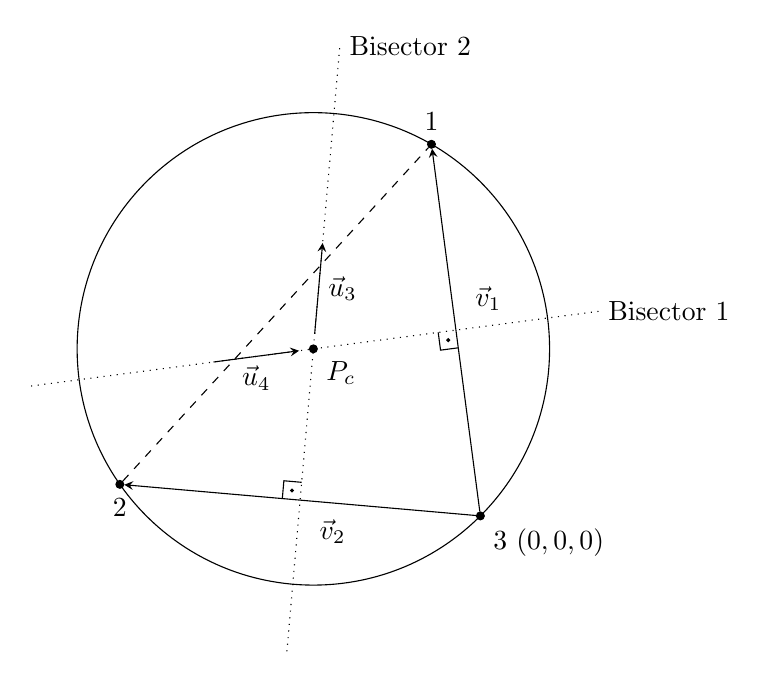
\begin{tikzpicture}
  [
    scale=3,
    >=stealth,
    point/.style = {draw, circle,  fill = black, inner sep = 1pt},
    dot/.style   = {draw, circle,  fill = black, inner sep = .2pt},
  ]

  % the circle
  \def\rad{1}
  \node (origin) at (0,0) [point, label = {below right:$P_c$}]{};
  \draw (origin) circle (\rad);

  % triangle nodes: just points on the circle
  \node (n1) at +(60:\rad) [point, label = above:$1$] {};
  \node (n2) at +(-145:\rad) [point, label = below:$2$] {};
  \node (n3) at +(-45:\rad) [point, label = {below right:$3$ $(0, 0, 0)$}] {};

  % triangle edges: connect the vertices, and leave a node at the midpoint
  \draw[->] (n3) -- node (a) [label = {above right:$\vec{v}_1$}] {} (n1);
  \draw[->] (n3) -- node (b) [label = {below right:$\vec{v}_2$}] {} (n2);
  \draw[dashed] (n2) -- (n1);

  % Bisectors
  % start at the point lying on the line from (origin) to (a), at
  % twice that distance, and then draw a path going to the point on
  % the line lying on the line from (a) to the (origin), at 3 times
  % that distance.
  \draw[dotted]
    ($ (origin) ! 2 ! (a) $)
    node [right] {Bisector 1}
    -- ($(a) ! 3 ! (origin)$ );

  % similarly for origin and b
  \draw[dotted]
    ($ (origin) ! 2 ! (b) $)
    -- ($(b) ! 3 ! (origin)$ )
    node [right] {Bisector 2};

  % short vectors
  \draw[->]
    ($ (origin) ! -.7 ! (a) $)
    -- node [below] {$\vec{u}_4$}
    ($ (origin) ! -.1 ! (a) $);
  \draw[->]
    ($ (origin) ! -.1 ! (b) $)
    -- node [right] {$\vec{u}_3$}
    ($ (origin) ! -.7 ! (b) $);

  % Right angle symbols
  \def\ralen{.5ex}  % length of the short segment
  \foreach \inter/\first/\last in {a/n3/origin, b/n2/origin}
    {
      \draw let \p1 = ($(\inter)!\ralen!(\first)$), % point along first path
                \p2 = ($(\inter)!\ralen!(\last)$),  % point along second path
                \p3 = ($(\p1)+(\p2)-(\inter)$)      % corner point
            in
              (\p1) -- (\p3) -- (\p2)               % path
              ($(\inter)!.5!(\p3)$) node [dot] {};  % center dot
    }
\end{tikzpicture}
%\end{document}
